\chapter{Eksperymenty}
\section{Wyniki ogólne}
Poniżej przedstawiono wynik działania algorytmu dla serii zdjęć zaprezentowanych w \ref{samples}.

\begin{figure}[H]
	\centering
		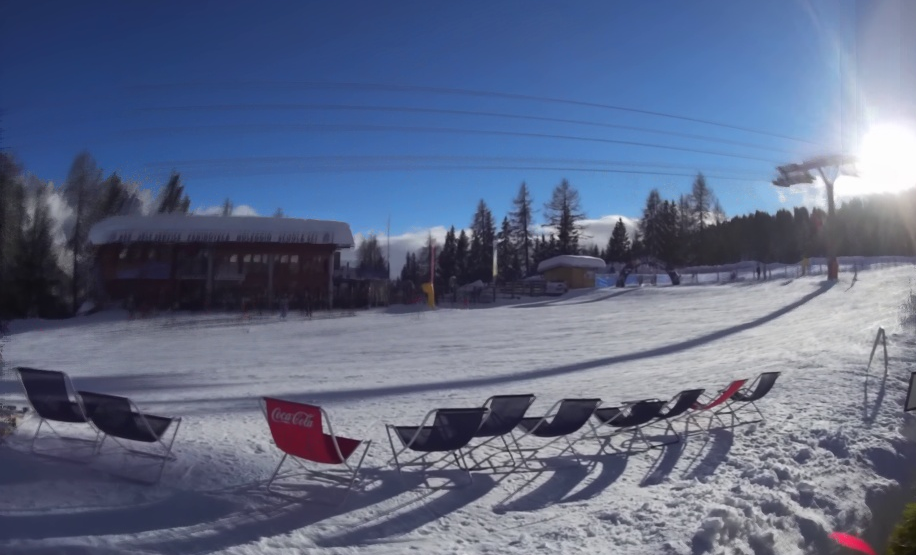
\includegraphics[width=1.0\linewidth]{img/ski_out.png}
	\caption[Wynika dla sekwencji zdjęć 'ski'.]{Wynika algorytmu dla sekwencji zdjęć 'ski'.}
	\label{fig:binary}
\end{figure}

Warto tutaj zwrócić uwagę na dosyć duże rozmazanie obrazu. Pomijając samą cechę algorytmu, który ma tendencję do rozmywania, tutaj efekt ten jest wyraźnie nasilony ze względu na dużą dystorsję soczewki aparatu. Brak eliminacji dystorsji w preprocessingu powoduje błędy w dopasowaniu poszczególnych zdjęć oraz złą sekwencję analizowanych pikseli co ma wyraźny wpływ na obraz wynikowy.

\begin{figure}[H]
	\centering
		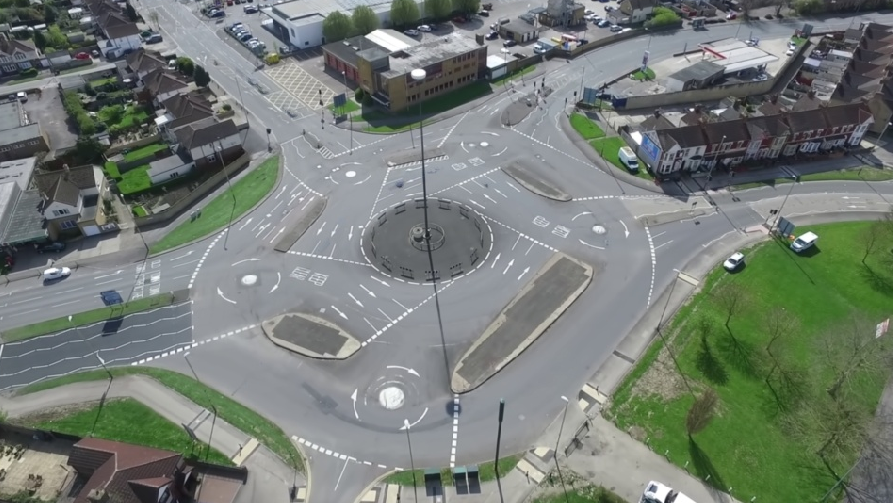
\includegraphics[width=1.0\linewidth]{img/roundabout_out.png}
	\caption[Wynika dla sekwencji zdjęć 'roundabout'.]{Wynika algorytmu dla sekwencji zdjęć 'roundabout'.}
	\label{fig:binary}
\end{figure}

Powyższy wynik jest jednym z najlepszych jakie udało się uzyskać. Jednym z powodów jest duża ilość zdjęć wejściowych - około 1000, dzięki czemu możliwe tak dokładne usunięcie wielu ruchomych pojazdów. Warto również zwrócić uwagę, że dopasowanie poszczególnych klatek miało istotny wpływ na efekt końcowy, gdyż zdjęcia wykonywane były za pomocą drona, którego pozycja ulegała delikatnej zmianie.

\begin{figure}[H]
	\centering
		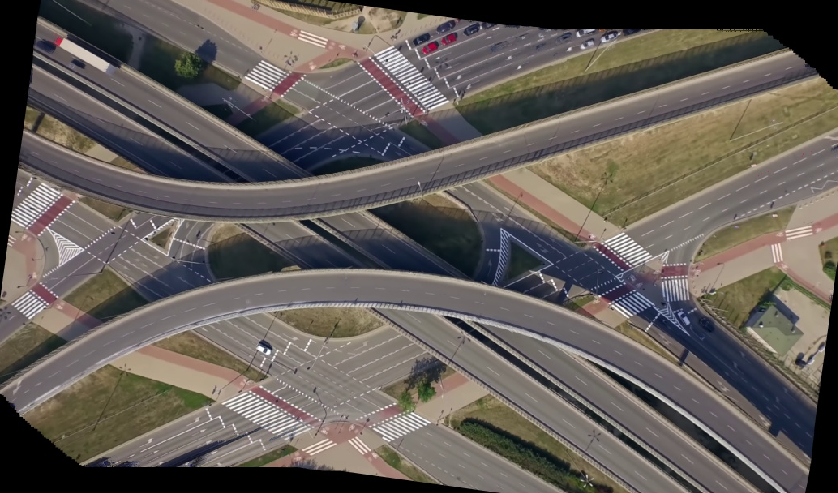
\includegraphics[width=1.0\linewidth]{img/warsaw_out.png}
	\caption[Wynika dla sekwencji zdjęć 'warsaw'.]{Wynika algorytmu dla sekwencji zdjęć 'warsaw'.}
	\label{fig:binary}
\end{figure}

W tym przypadku dopasowanie kolejnych klatek miało szczególne znaczenie, ze względu na dosyć duży obrót kamery. W górnej części obrazu widać pewne artefakty powstałe po usunięciu części obrazu. Błędy te spowodowane są małą ilością klatek składowych, które znalazły się w przetwarzanej sekwencji oraz niskim podobieństwem pomiędzy kolejnymi obrazami (mała ilość części wspólnych).

\begin{figure}[H]
	\centering
		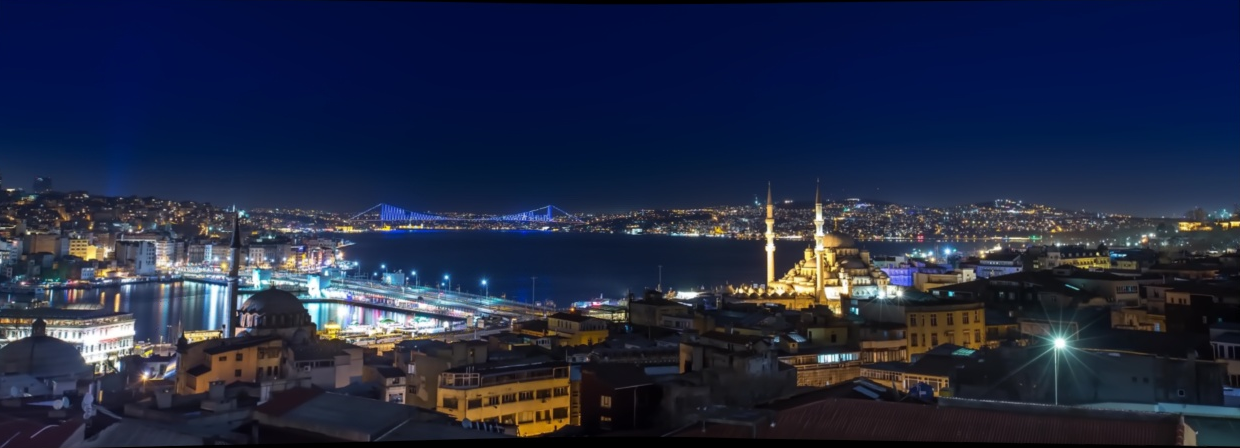
\includegraphics[width=1.0\linewidth]{img/istanbul_out.png}
	\caption[Wynika dla sekwencji zdjęć 'istanbul'.]{Wynika algorytmu dla sekwencji zdjęć 'istanbul'.}
	\label{fig:binary}
\end{figure}

Panoramiczne ujęcie otrzymane za pomocą zaproponowanego algorytmu. Zauważalne rozmycie obrazu spowodowane jest również kompresją poszczególnych ujęć składowych (kompresja jpeg). Szumy powstałe na krawędziach mają istotny wpływ na efekt końcowy.

\section{Wyniki szczegółowe}
\subsection{Dopasowanie obrazów}

\begin{figure}[H]
\centering
\begin{subfigure}{.5\textwidth}
  \centering
  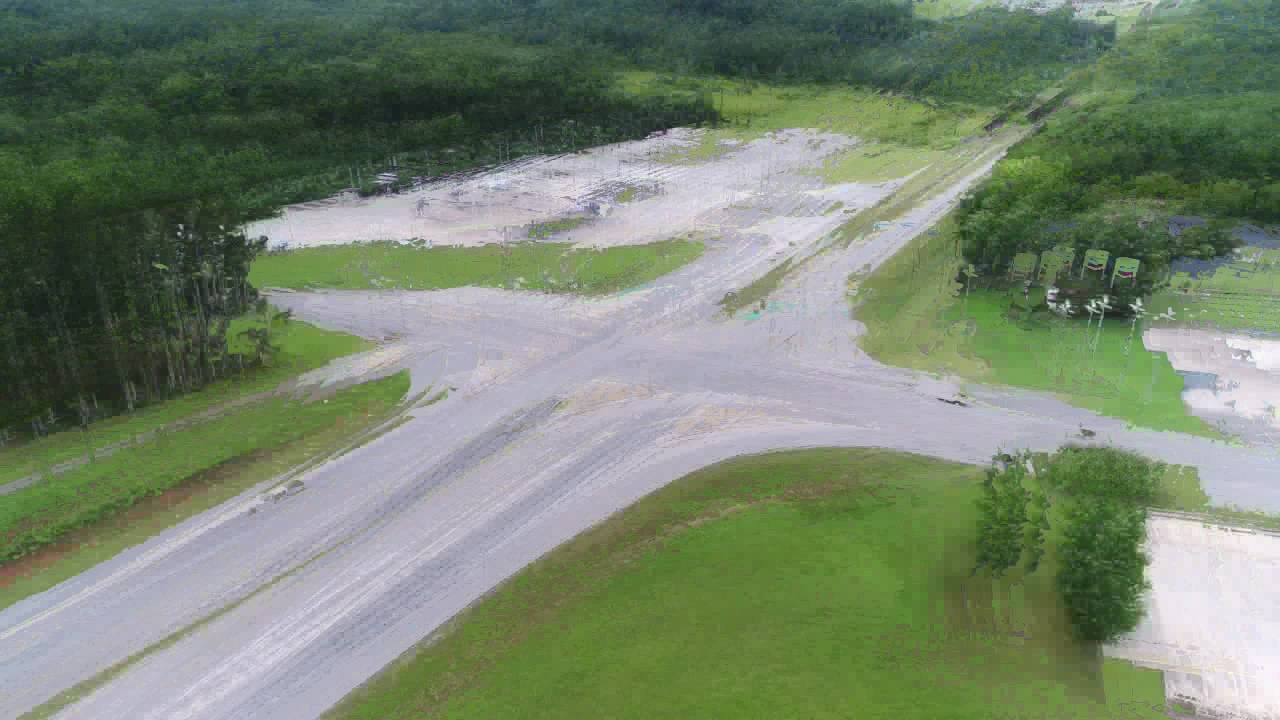
\includegraphics[width=.95\linewidth]{img/non-match.png}
  \caption{Brak dopasowania}
  \label{fig:sub1}
\end{subfigure}%
\begin{subfigure}{.5\textwidth}
  \centering
  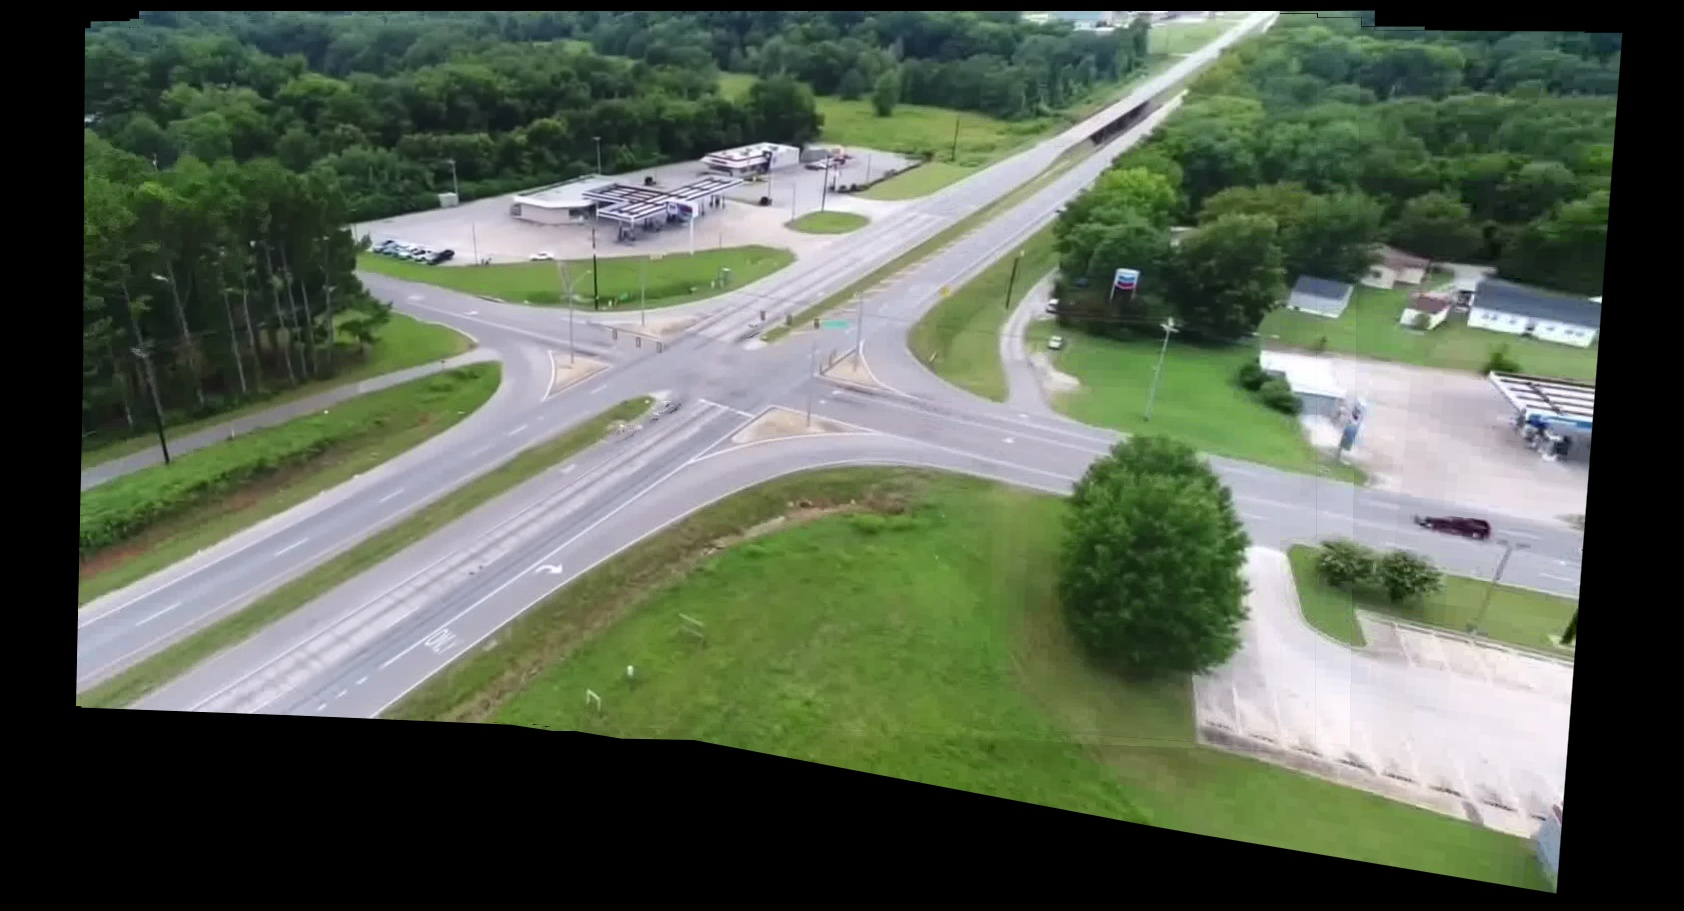
\includegraphics[width=.95\linewidth]{img/match.png}
  \caption{Z dopasowaniem}
  \label{fig:sub2}
\end{subfigure}
\caption{Porównanie wykonania algorytmu z dopasowaniem obrazów.}
\label{fig:test}
\end{figure}
Na powyższym przykładzie pokazano jak duży wpływ na efekt końcowy ma sprowadzenie każdej klatki do wspólnej przestrzeni współrzędnych. Oczywiście brak dopasowania ruchomego obrazu to skrajny przypadek, ale warto zwrócić uwagę, że niewielkie odchylenia mogą powodować artefakty lub efekty rozmycia.
\subsection{Przestrzeń barw}
\begin{figure}[H]
\centering
\begin{subfigure}{.5\textwidth}
  \centering
  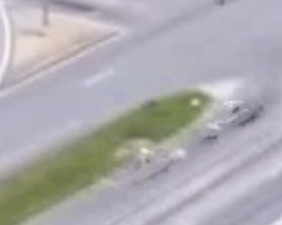
\includegraphics[width=.95\linewidth]{img/bgr-art.png}
  \caption{Przestrzeń barw BGR}
  \label{fig:sub1}
\end{subfigure}%
\begin{subfigure}{.5\textwidth}
  \centering
  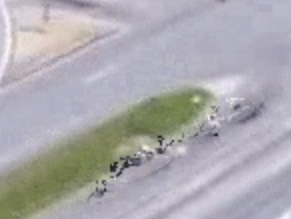
\includegraphics[width=.95\linewidth]{img/hls-art.png}
  \caption{Przestrzeń barw HLS}
  \label{fig:sub2}
\end{subfigure}
\caption{Porównanie wykonania algorytmu z dla różnych przestrzeni barw.}
\label{fig:bgrhls}
\end{figure}

Rysunek \ref{fig:bgrhls} przedstawia szczegółowe artefakty powstałe przy przetwarzania za pomocą różnych przestrzeni barw. Na poziomie poszczególnych pikseli widoczne są pewne błędy przetwarzania. W tym przypadku przestrzeń barw HLS uzyskała odrobinę gorszy wynik niż BGR. Nie jest to jednak regułą, a dobór odpowiedniej przestrzeni jest mocno zależny od dalszych etapów przetwarzania oraz samej charakterystyki obrazów wejściowych.
\subsection{Wartości piksela}
\begin{figure}[H]
\centering
\begin{subfigure}{.333\textwidth}
  \centering
  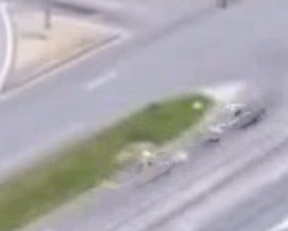
\includegraphics[width=.95\linewidth]{img/channel-art.png}
  \caption{Jeden z kanałów.}
\end{subfigure}%
\begin{subfigure}{.333\textwidth}
  \centering
  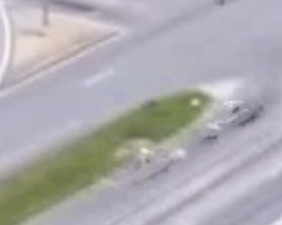
\includegraphics[width=.95\linewidth]{img/bgr-art.png}
  \caption{Długość wektora}
\end{subfigure}%
\begin{subfigure}{.333\textwidth}
  \centering
  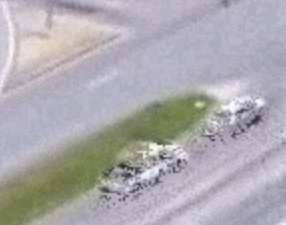
\includegraphics[width=.95\linewidth]{img/vec-art.png}
  \caption{Suma różnic wektrów}
  \label{fig:vec}
\end{subfigure}%
\caption{Porównanie wykonania algorytmu dla różnych metod liczenia wartości pikseli.}
\label{fig:value}
\end{figure}

Powyżej (rys. \ref{fig:value}) zaprezentowano artefakty powstałe ze względu na metodę liczenia wartości piksela. Podobnie jak poprzednio nie można jednoznacznie stwierdzić która z nich daje lepsze wyniki, gdyż wpływa na to wiele czynników. Warto jednak zauważyć, że metoda wektorowa (rys. \ref{fig:vec}) wyraźnie różni się od pozostałych i daje dosyć wyraźne szumy.